\begin{frame}{Benchmark models}
\framesubtitle{Analyzing the prediction importance of literature features alone}

\begin{columns}
    \begin{column}{0.25\textwidth} 
    First, we trained the outcome prediction models using only the best-known genes consolidated by studies in the literature, both for the expression and mutation contexts.
    \end{column}

    \begin{column}{0.7\textwidth}
        
\small

\begin{table}[!htb]
    \centering
    %
    \label{tab:literature-results}    
        \begin{tabular}{llrrrrr}
        \toprule
        Model &  F1-Score &       AUC &  Accuracy &  Precision &    Recall \\
        \midrule
        CLIN                       &  0.57 &  0.53 &  0.57 &   0.57 &  0.57 \\
        MUT                       &  0.64 &  \textbf{0.70} &  0.64 &   \textbf{0.76} &  0.64 \\
        EXP                        &  0.66 &  0.62 &  \textbf{0.68} &   0.66 &  \textbf{0.68} \\
        CLIN+MUT           &  \textbf{0.67} &  0.64 &  \textbf{0.68} &   0.67 &  \textbf{0.68} \\
        CLIN+EXP            &  0.57 &  0.53 &  0.57 &   0.57 &  0.57 \\
        MUT+EXP             &  0.63 &  0.59 &  0.64 &   0.63 &  0.64 \\
        CLIN+MUT+EXP &  0.54 &  0.51 &  0.54 &   0.55 &  0.54 \\
       
        \bottomrule
        \end{tabular}
        \caption{Results achieved by the outcome prediction models. The genes from MUT and EXP were selected according to consolidated studies in the literature}
\end{table}
    \end{column}

    
\end{columns}
\end{frame}



%\begin{itemize}
 %   \item The model that achieved the best result was the one that combined clinical and genetic mutation data;
  %  \item When analyzing the models trained with individual datasets, the ones based on gene mutation and expression showed the best performances;
   % \item The overall results obtained are low and unsatisfactory for predicting the outcomes of AML patients;
    %\item The genes most known in the literature seem not strongly associated with outcomes prediction.
%\end{itemize}


\begin{frame}{Training the EBMs}
\framesubtitle{Training the models with the selected features}

\begin{columns}
    \begin{column}{0.25\textwidth} 
    We then trained the outcome prediction models using the data resulting from the pre-processing, data analysis, and feature selection process described before.
    \end{column}

    \begin{column}{0.7\textwidth}
        
\small

\begin{table}[htb!]
    \centering
   
    \label{tab:all-results}    
    \begin{tabular}{llrrrrr}
        \toprule
        Model &  F1-Score & AUC &  Accuracy &  Precision &    Recall \\
        \midrule
        CLIN                        &  0.57 &  0.53 &  0.57 &   0.57 &  0.57 \\
        MUT                         &  0.65 &  0.63 &  0.64 &   0.66 &  0.64 \\
        EXP                           &  \textbf{0.86} &  \textbf{0.84} &  \textbf{0.86} &   \textbf{0.86} &  \textbf{0.86} \\
        CLIN+MUT              &  0.67 &  0.64 &  0.68 &   0.67 &  0.68 \\
        CLIN+EXP                &  0.78 &  0.74 &  0.79 &   0.78 &  0.79 \\
        MUT+EXP                &  0.82 &  0.79 &  0.82 &   0.82 &  0.82 \\
        CLIN+MUT+EXP     &  0.78 &  0.74 &  0.79 &   0.78 &  0.79 \\
      
        \bottomrule
    \end{tabular}
     \caption{Results achieved by the outcome prediction models. The genes from MUT were selected using $\chi^2$-test + the genes selected according to the literature.  The genes from EXP were selected using LASSO}
    \end{table}
    \end{column}

    
\end{columns}
\end{frame}



%The performance of the model trained only with the mutation data deteriorated slightly compared to the one obtained only with the genes highlighted in the literature. However, the performance of the model trained only with the expression data showed a remarkable improvement since all performance measures were up about 30\%, and figuring as the best model we achieved. This strong increase in model performance is probably due to the careful KDD (Knowledge Discovery in Databases) process performed on the data and the new genes discovered to be good predictors.


%The main advantage of using EBMs is that they are highly intelligible because the contribution of each feature to an output prediction can be easily visualized and understood.
%Figure~\ref{fig:prediction-interpretability} shows the local explanation for two test samples correctly classified as positive and negative using the classification model trained with the EXP feature set.

\begin{frame}{Interpreting the results -  Positive prediction}
\framesubtitle{Understanding the importance of features}
        \begin{figure}[!htb]
    \begin{center}
        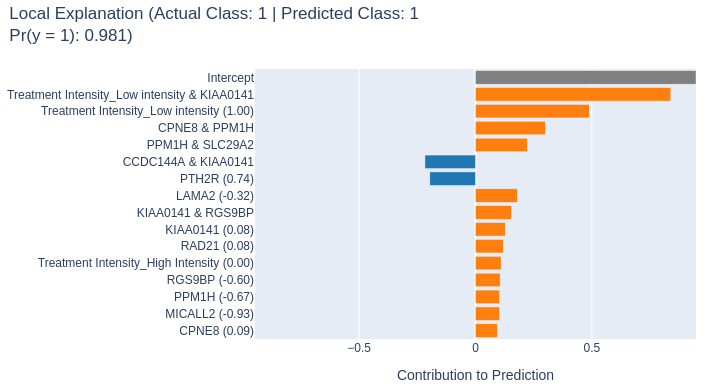
\includegraphics[width=0.6\textwidth]{beamerthemesrc/figs/TP_prediction.png}
    \end{center}
    \caption{\tiny Local explanation for a single sample using then model trained with the EXP feature set. The intercept reflects the average case presented as a $log$ of the base rate (e.g., $-2.3$ if the base rate is $10\%$). The 15 most important terms are shown.}
    \label{fig:prediction-interpretability}
\end{figure}
    
\end{frame}



\begin{frame}{Interpreting the results - Negative prediction}
\framesubtitle{Understanding the importance of features}


\begin{figure}[!htb]
    \begin{center}
        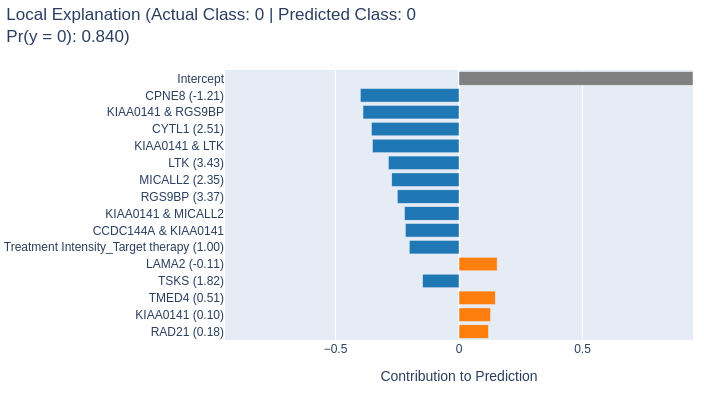
\includegraphics[width=0.6\textwidth]{beamerthemesrc/figs/TN_prediction.png}
    \end{center}
    \caption{\tiny Local explanation for a single sample using then model trained with the EXP feature set. The intercept reflects the average case presented as a $log$ of the base rate (e.g., $-2.3$ if the base rate is $10\%$). The 15 most important terms are shown.}
    \label{fig:prediction-interpretability}
\end{figure}

\end{frame}


%Figure~\ref{fig:feature-importance} presents the top-15 attributes according to their importance in generating the prediction of outcome using gene mutation (Fig~\ref{fig:feat_imp_MUT}), gene expression (Fig~\ref{fig:feat_imp_EXP}), and clinical data (Fig~\ref{fig:feat_imp_CLIN}), respectively. The attribute importance scores represent the average absolute contribution of each feature or interaction to the predictions, considering the entire training set. These contributions are weighted based on the number of samples within each group.




\begin{frame}{Interpreting the results - CLIN}
\framesubtitle{Understanding the importance of features}
    
\begin{figure}[!htbp]
    \centering
         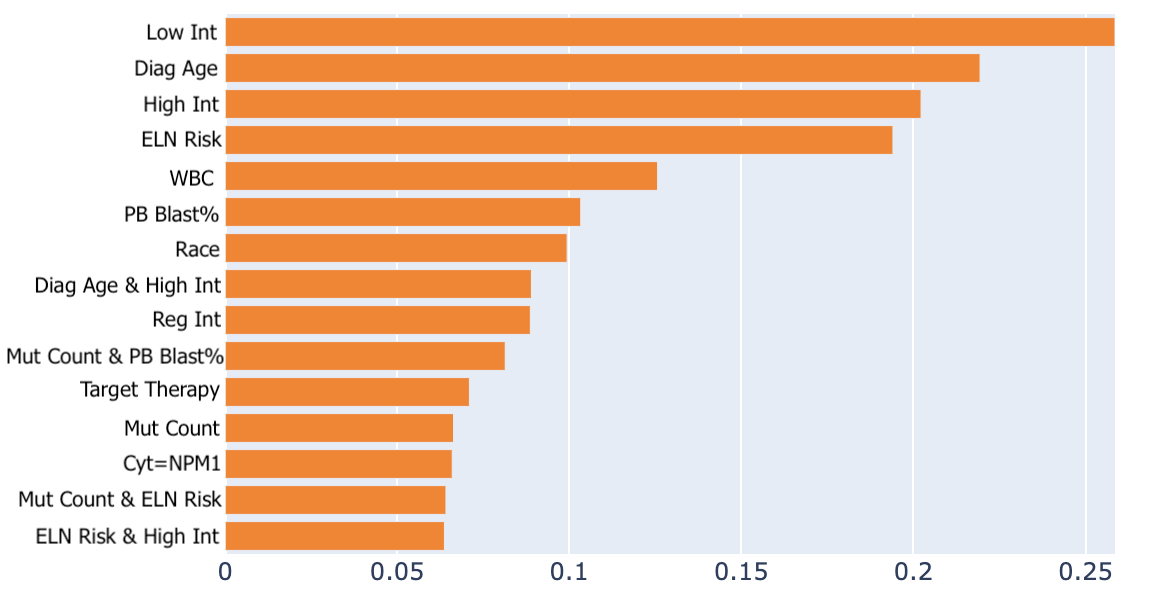
\includegraphics[width=.65\textwidth]{beamerthemesrc/figs/feat_importance_CLIN.png}
         \label{fig:feat_imp_CLIN}
    \caption{Top-15 features that most influence the models' prediction (CLIN)}
    \label{fig:feature-importance}
    \end{figure}

\end{frame}


\begin{frame}{Interpreting the results - MUT}
\framesubtitle{Understanding the importance of features}
    
\begin{figure}[!htbp]
    \centering
         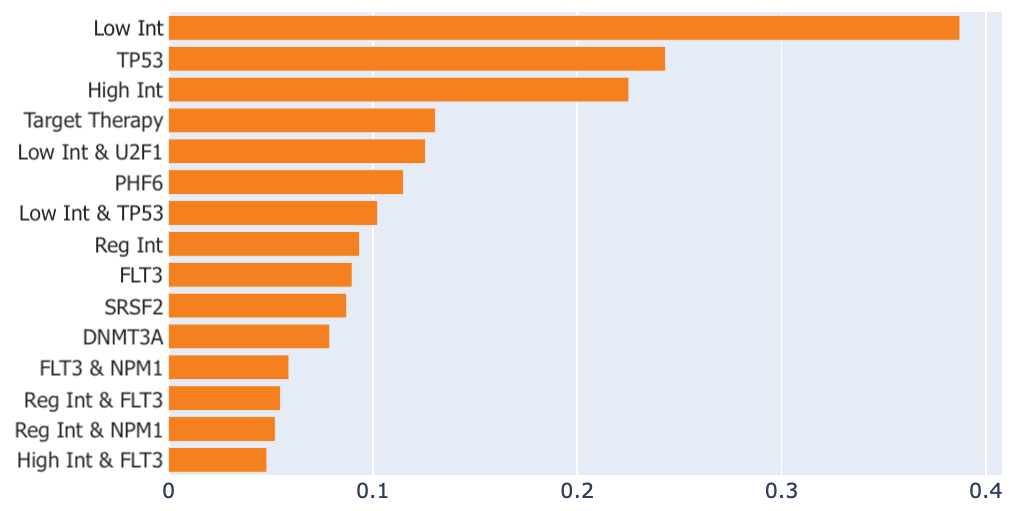
\includegraphics[width=.65\textwidth]{beamerthemesrc/figs/feat_importance_MUT.png}
         \label{fig:feat_imp_MUT}
    \caption{Top-15 features that most influence the models' prediction (MUT)}
    \label{fig:feature-importance}
    \end{figure}

\end{frame}



\begin{frame}{Interpreting the results - EXP}
\framesubtitle{Understanding the importance of features}
    
\begin{figure}[!htbp]
    \centering
         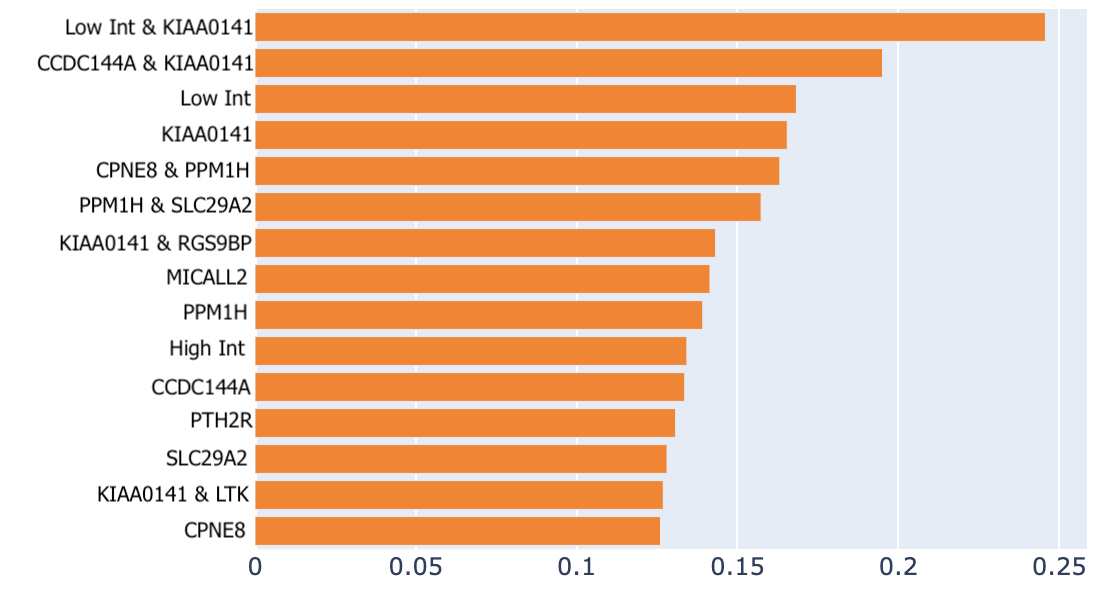
\includegraphics[width=.65\textwidth]{beamerthemesrc/figs/feat_importance_EXP.png}
         \label{fig:feat_imp_EXP}
    \caption{Top-15 features that most influence the models' prediction (EXP)}
    \label{fig:feature-importance}
    \end{figure}

\end{frame}







%\begin{frame}{Our findings}

%\begin{itemize}
  
%\item The four most influential clinical features are: \emph{low-intensity treatment, the patient's age, high-intensity treatment and the ELN risk classification};
%\item  It is well-known that the age at diagnosis and the ELN risk classification can potentially impact the patient's outcome \cite{Dohner-2022}.

%\item Among the gene mutation features, \emph{PHF6} and \emph{TP53} ranked the highest, followed by the gene mutations already well-known in the literature;

%\item Among the most influential genetic expression features for model prediction, the following stand out \textit{KIAA0141}, \textit{MICALL2}, and \textit{SLC9A2}, for which there are few studies in the literature in the context of AML;
    %\item The gene \textit{KIAA0141} has been recently identified as a key player~\cite{Sharon-2023}. Research suggests that dysregulation of the expression of this gene contributes to the inactivation of the integrated stress response in patients with TP53 gene mutations;

    %\item In a pan-cancer analysis, \textit{MICALL2} was highly expressed in 16 out of 33 cancers compared to normal tissues~\cite{lin-2022-35281853};

    %\item   The role of \textit{SLC9A2} in cancer is still an area of active research, and the exact relationship between \textit{SLC9A2} and cancer development or progression is not fully understood.
    
%\end{itemize}
%\end{frame}


 %However, some studies have suggested potential associations between \textit{SLC9A2} and certain types of cancer, such as colorectal, breast, and gastric cancer.

%The findings presented in this paper suggest that the biological role of these genes in the pathogenesis and progression of AML deserves future functional studies in experimental models and may provide insights into the prognosis and the development of new treatments for the disease.

 


%Considering that specialists often do not have access to the most suitable treatment intensity during model prediction, the predictions are automatically generated for the four categorized treatment types (Section \ref{subsec:datasets}), and the one that best optimizes the patient's survival time is selected as the recommended therapy.


%Regarding genetic mutation data, the mutations in the \textit{TP53} and \textit{PHF6} genes are ranked as the most influential, followed by the gene mutations already well-known in the literature. If, on the one hand, the mutation in the \textit{TP53} gene was already expected, to the best of our knowledge, there are no studies in the literature associating the \textit{PHF6} gene with predicting outcomes in the context of AML. Therefore, laboratory tests should be performed to confirm whether this gene may serve as a potential prognostic marker.